\documentclass[twocolumn, a4paper]{extarticle}
\usepackage{fontspec}   %加這個就可以設定字體
\usepackage{xeCJK}       %讓中英文字體分開設置
\usepackage{listings}
\usepackage[newfloat]{minted}
\usepackage{float}
\usepackage{graphicx}
\usepackage{caption}
\usepackage{fancyhdr}
\usepackage{hyperref}
\usepackage{amsmath}
\usepackage{multirow}
\usepackage[dvipsnames]{xcolor}
\usepackage{graphicx}
\usepackage{tabularx}
\usepackage{booktabs}
\usepackage{caption}
\usepackage{subcaption}
\usepackage{pifont}
\usepackage{amssymb}
\usepackage{titling}

\usepackage{pdftexcmds}
\usepackage{catchfile}
\usepackage{ifluatex}
\usepackage{ifplatform}

\usepackage[breakable, listings, skins, minted]{tcolorbox}
\usepackage{etoolbox}
\setminted{fontsize=\footnotesize}
\renewtcblisting{minted}{%
    listing engine=minted,
    minted language=python,
    listing only,
    breakable,
    enhanced,
    minted options = {
        linenos, 
        breaklines=true, 
        breakbefore=., 
        % fontsize=\footnotesize, 
        numbersep=2mm
    },
    overlay={%
        \begin{tcbclipinterior}
            \fill[gray!25] (frame.south west) rectangle ([xshift=4mm]frame.north west);
        \end{tcbclipinterior}
    }   
}

\usepackage[
top=1.5cm,
bottom=0.75cm,
left=1.5cm,
right=1.5cm,
includehead,includefoot,
heightrounded, % to avoid spurious underfull messages
]{geometry} 

\usepackage[
backend=biber,
style=ieee,
natbib=true,
doi=true,
eprint=false
]{biblatex}

\addbibresource{report.bib}


\newenvironment{code}{\captionsetup{type=listing}}{}
\SetupFloatingEnvironment{listing}{name=Code}
\usepackage[moderate]{savetrees}


\title{AI Capstone Final Project \\ Using Different Methods to Solve TSP}
\author{110550088 李杰穎、110652019 林楷傑、110950011 廖家淯}
\date{\today}


\setCJKmainfont{Noto Serif TC}


\ifwindows
\setmonofont[Mapping=tex-text]{Consolas}
\fi

\XeTeXlinebreaklocale "zh"             %這兩行一定要加,中文才能自動換行
\XeTeXlinebreakskip = 0pt plus 1pt     %這兩行一定要加,中文才能自動換行

% \setlength{\parindent}{0em}
\setlength{\parskip}{0.75em}
\renewcommand{\baselinestretch}{1.15}
\setlength{\droptitle}{-10em}   % This is your set screw
\setlength{\columnsep}{2em}

\begin{document}

\maketitle

\section{Background Overview}

The Traveling Salesman Problem (TSP) is a well-known optimization problem in the field of computer science and mathematics. It belongs to the category of NP-hard problems, which means that finding an optimal solution becomes increasingly difficult as the problem size increases.

The problem is defined as follows: given a list of cities and the distances between each pair of cities, the task is to find the shortest possible route that visits each city exactly once and returns to the starting city. The objective is to minimize the total distance traveled.

The TSP has been extensively studied since its introduction in the 1930s and has applications in various fields such as logistics, transportation planning, circuit board drilling, and DNA sequencing. Its name was inspired by the analogy to a traveling salesman who needs to find the shortest route to visit a set of cities and return to the starting point.

One of the reasons why the TSP is of great interest to researchers is its computational complexity. As the number of cities increases, the number of possible routes grows factorially, resulting in an exponential increase in computational effort required to find the optimal solution. For large problem instances, it becomes practically impossible to explore all possible solutions.

In summary, the Traveling Salesman Problem is a classic optimization problem that seeks to find the shortest route visiting a set of cities and returning to the starting point. Its computational complexity has driven the development of various algorithms and approaches, making it a fundamental problem in the fields of computer science and mathematics.


\section{Selected Paper}

In this project, we used three methods to solve TSP, including ant colony optimization (ACO), deep reinforcement learning (DRL) and firefly algorithm. In this section, we will explain these three methods and their correspond papers respectively.

\subsection{ACO}

For ACO, we mainly referenced \cite{stutzle1999aco}, this paper is a overview of using ACO to solve TSP. It introduced three methods of ACO, we will introduce these three methods.

\subsubsection{Introduction}
Ant Colony Optimization (ACO) is widely used to solve NP-hard optimizing problem, in particular, TSP problem. In the paper, the authors introduced three different ant system methods, including ant system (AS), ant colony system (ACS) and MAX-MIN ant system (MMAS). I will breifly explain how these methods work in the next few sections.

However, because of the complexity of implementation and the fact that MMAS is a improved version of AS, I will only implement MMAS, and only MMAS will be compared with DRL and firefly algorithm.

Before explaining the two methods, I will first introduce the concept of ant system. Ant system is inspired by the behavior of real ant colony. When ants are finding the shortest path from nest to food, they would spread pheromone along the path, so that other ants can follow the path to get the food. Because pheromone can evaporate, after time, longer path will get less pheromone, thus less attractive to other ants. Therefore, after period of time, the ant colony will find the shortest path eventually. 

Ant system used artificial pheromone and ants to simulate the behavior of real ant. The pheromone some how reflect their experience while solving a particular problem.

The below notations will be used in the two methods.

\begin{itemize}
	\item $\tau_{ij}(t)$ is the pheromone strength of arc $(i, j)$ in $t$ iteration
	\item $d_{ij}$ is the distance from city $i$ to $j$
	\item $\eta_{ij}(t)$ is the priori available heuristic value of arc $(i, j)$. Usually set to $1/d_{ij}(t)$
\end{itemize}


Noted that in this project all the TSP problems are symmetric, i.e. $d_{ij}(t) = d_{ji}(t)$. Therefore, $\tau_{ij}(t)$ is also symmetric, i.e. $\tau_{ij}(t) = \tau_{ji}(t)$.

\subsubsection{AS}

The are mainly three variants of AS, ant-density, ant-quantiy and ant-cycle. The first two methods update pheromone right after a move from a city to adjacent one. The ant-cycle AS update pheromone after a full tour is completed. Because ant-cycle AS perform much better than the other two variants, the paper used ant-cycle variants.

In AS, each $m$ artifical ants construct a solution to TSP. Noted that local search doesn't apply to original AS.

\textbf{Tour Construction} Initially, each $m$ artificial ants put randoml chosen city. At each construction step, ant $k$ choose the next traverse city by the probability describe as follow:

\begin{equation}
	p_{i j}^k(t)=\frac{\left[\tau_{i j}(t)\right]^\alpha \cdot\left[\eta_{i j}\right]^\beta}{\sum_{l \in \mathcal{N}_i^k}\left[\tau_{i l}(t)\right]^\alpha \cdot\left[\eta_{i l}\right]^\beta} \quad \text { if } j \in \mathcal{N}_i^k
	\label{eq: choice}
\end{equation}

We can notice that the arc with more phermone or shorter distance will have more chance to be traversed, and $\mathcal{N}_i^k$ is the is the feasible neighborhood of ant $k$, that is, the set of cities which ant $k$ has not yet visited. We can also noticed that if $\alpha=0$, the closest cities are more likely to be selected. And if $\beta=0$ only pheromone amplification is at work: this method will lead to the rapid emergence of a stagnation situation with the corresponding generation of tours which, in general, are strongly suboptimal.

\textbf{Pheromone update} After all ants have constructed their tours, the pheromone trails are updated. This is done by first lowering the pheromone strength on all arcs by a constant factor and then allowing each ant to add pheromone on the arcs it has visited:

\begin{equation}
	\tau_{i j}(t+1)=(1-\rho) \cdot \tau_{i j}(t)+\sum_{k=1}^m \Delta \tau_{i j}^k(t)
\end{equation}

, where $0 < \rho \leq 1$ is the pheromone trail evaporation rate. With evaporation, the algorithm can ``forget'' previous done bad decisions. And the $\Delta \tau_{i j}^k(t)$ here is defined as:

\begin{equation}
	\Delta \tau_{i j}^k(t)=\left\{\begin{array}{cl}
		1 / L^k(t) & \text { if } \operatorname{arc}(i, j) \text { is used by ant } k \\
		0 & \text { otherwise }
	\end{array}\right.
\end{equation}

$L^k(t)$ is the path distance of ant $k$ in $t$ iteration.

By \textbf{Tour Construction} and \textbf{Pheromone Update}, the AS algorithm can approach optimal value after iterations. However, AS often fall into local optimal value, thus can't achieve good solution. To overcome this situation, the later researcher used ACS instead. 

\subsubsection{MMAS}

MIN-MAX ant system (MMAS) is also a improved AS. Not like ACS, the implementation of MMAS is very similar to AS. The solutions in MMAS are constructed in exactly the same way as in AS, that is, the selection probabilities are calculated as in \autoref{eq: choice}. 

The main modification of MMAS is that it adopted the lower and upper bound for pheromone level, the lower and upper bound is denoted as $\tau_{min}$ and $\tau_{max}$ respectively. After pheromone update, any value that is smaller than $\tau_{min}$ will be increased to $\tau_{min}$ and any value that is greater than $\tau_{max}$ will be decreased to $\tau_{max}$. In this way, we can avoid that ants fall into local optimal, with each cities has relatively higher chance to be traversed compared with original AS.

Below are the actual steps of MMAS.

\textbf{Update of pheromone trails.} Like in AS, after all the ants constructed a path, the pheromone is updated as follow:

\begin{equation}
	\label{eq: mmas}
	\tau_{i j}(t+1)=(1-\rho) \cdot \tau_{i j}(t)+\sum_{k=1}^m \Delta \tau_{i j}^{best}(t)
\end{equation}

, where $\tau_{i j}^{best}(t) = \frac{1}{L^{best}}$. The $L^{best}$ here is either global best solution $T^{gb}$ or iteration best solutions $T^{ib}$. In the experiments, we will set $L^{best}$ to one of these two solution by a schedule. By experiments, the authors of \cite{stutzle1999aco} mentioned that gradually increased the frequency of choosing $T^{gb}$ yields a better solution. The detail of scheduler will be explained in the experiment section.

\subsubsection{Local Search of Ants}

To better improved the performance of MMAS, the authors suggests that we can apply local search algorithm to a constructed path. This will make the solution better.

A popular local search algorithm is \texttt{2-opt}. \texttt{2-opt} enumerates all possible pair of cities, and swap the order of these two cities in the path, and check if the distance of the swapped path decreased for a given percentage. After applying \texttt{2-opt} the solution of MMAS is far better, and the convergence speed is also increased.


\subsection{Firefly Algorithm}

\subsubsection{Introduction}
Firefly Algorithm got the idea from how fireflies synchronize their lights. In this paper, the author use Firefly Algorithm to solve the TSP problem and could converge to the optimal solution faster than PCO for some specific problems. This algorithm is introduced in \cite{jati2011evolutionary}.

\subsubsection{Firefly}
Each firefly represent a solution to the TSP problem, the solution is represented by the order of the city to travel.

For example, if there are 5 cities labeled with number 0 to 4, than the firefly (0, 2, 4, 1, 3) means the salesman travels to city 0, 2, 4, 1, 3 and goes back to city 0.

\subsubsection{Distance}
The distance of two firefly is defined by the total number of different arcs. 

For example, the distance between fireflyA (0, 1, 2, 3, 4) and fireflyB (0, 1, 3, 2, 4) is 2, since arc 1->2 and 2->3 in fireflyA is not in fireflyB.

\subsubsection{Attractiveness}
The attractiveness of fireflyA to fireflyB is defined by the following formula, where $r$ is the distance between fireflyA and fireflyB.
\begin{equation}
	\beta(r)=\beta_0e^{-\gamma r^2}
\end{equation}


$\gamma$ is called light absorption factor and can be used to control how much a firefly can affect others. if $\gamma$ is set to 0, all firefly have the same attractiveness regardless near or far, and if $\gamma$ is set to $\infty$ than all firefly will have no affect on others.

\subsubsection{Movement}
In each iteration in firefly algorithm, each firefly will "move" toward the most attractive firefly.
In this paper, since a firefly means a solution of the TSP problem, so the firefly is moving in the solution space. 

The movement of fireflyA to another fireflyB is determined by

\begin{equation}
	\beta(r)=\beta_0e^{-\gamma r^2}
\end{equation}

where $x_A$ is the length of movement, and $r_{AB}$ is the distance between fireflyA and fireflyB and scale into the range of [0, 10].

Than we randomly select a index in fireflyA's solution and perfrom Inverse Permutation with length $x_A$.

\subsection{DRL}

\subsubsection{Introduction}

DQN, or Deep Q-Network, is a reinforcement learning algorithm that combines deep learning and Q-learning to solve complex decision-making problems. It first appears in \cite{mnih2013playing}. At its core, DQN leverages a deep neural network to estimate the Q-values of different actions in a given state. The Q-values represent the expected future rewards for taking a particular action in a specific state. By learning these values, the agent can make informed decisions on which actions to take to maximize its cumulative reward. 

The DQN algorithm uses a technique called experience replay, which stores the agent's experiences (state, action, reward, next state) in a replay memory. During training, the agent samples mini-batches of experiences from this memory to decorrelate the data and improve learning efficiency.

The learning process of DQN can be summarized using the following equation:

\begin{equation}
	Q(s, a) \leftarrow (1 - \alpha) \cdot Q(s, a) + \alpha \cdot (r + \gamma \cdot \max_{a'} Q(s', a'))
\end{equation}

Here, $Q(s, a)$ represents the estimated Q-value of action $a$ in state $s$. The algorithm updates this estimate using a weighted average of the current estimate $(1 - \alpha) \cdot Q(s, a)$ and a new estimate $\alpha \cdot (r + \gamma \cdot \max_{a'} Q(s', a'))$. In this equation, $r$ represents the immediate reward obtained after taking action $a$ in state $s$, $s'$ represents the resulting state, $\alpha$ is the learning rate, and $\gamma$ is the discount factor that determines the importance of future rewards.

By repeatedly updating the Q-values based on this equation, DQN gradually learns to approximate the optimal Q-function, which leads to better decision-making capabilities for the agent.


\subsubsection{RL Environment}

For the graph $G(V, E)$, $N = |V|$.

\begin{itemize}
	\item State representation
	
	State representation is Nx5 vector, where for each node we store whether this node is in the sequence, whether it is first or last, and its (x,y) coordinates. The coordinates of each nodes have normalize to one, for the sake of convenience of training neural net.
	\item Action
	
	The action is the integer from 1 to N. The env will mask the nodes that have been visited. The solution list is a list contained the nodes that have been visited.
	\item Reward definition
	
	The reward is calculated based on the total distance traveled by the solution compared to the current solution. \texttt{reward = -(total\_dist(next\_solution) - total\_dist(solution))}

\end{itemize}

\subsubsection{Deep Neual Network Design}
The network consists of five fully connected (dense) layers (hidden size is 1600) with ReLU activation applied to the output of each layer except for the last one. The input dimension is defined by shape of state tensor, the number of actions is defined by total number of nodes, and the size of the hidden layers is set to \texttt{hidden\_layer\_size}. The network takes input states and produces corresponding Q-values, which are used to estimate the value of each action in a reinforcement learning context.


\section{Experiments and Findings}

\subsection{Problem Instances}

In this project, we used the TSP from TSPLIB \cite{reinelt1991tsplib}. These problems already has optimal solutions. Thus, it's easier to compare with the solution generated by the three methods.

We pick five problem instances, the name and optimal solution can be found in \autoref{tab: tsplib}. Noted that this five TSP is relatively small problem size, because we afraid that large TSP will make the running of algorithm increased.

\begin{table}[H]
	\caption{The five chosen TSP instances from TSPLIB.}
	\label{tab: tsplib}
	\begin{tabular}{@{}ccc@{}}
		\toprule
		\textbf{Problem} & \textbf{Number of Cities} & \textbf{Optimal Solution} \\ \midrule
		berlin52         & 52                        & 7542                      \\
		rat99            & 99                        & 1211                      \\
		bier127          & 127                       & 118282                    \\
		ch130            & 130                       & 6110                      \\
		a280             & 280                       & 2579                      \\ \bottomrule
	\end{tabular}
\end{table}

\subsection{Parameters in Experiments}

In this section, we list the parameters used in the experiments.

\subsubsection{ACO}

The method we used in ACO is MMAS, the parameters of MMAS is as follow:

\begin{itemize}
	\item Number of ants = 100
	\item Max iterations = 500
	\item $\alpha=1$
	\item $\beta=2$
	\item $\rho=0.2$
	\item Every ants runs \texttt{2-opt} right before update pheromone
	\item $\tau_{max} = \frac{1}{\rho T^{gb}}$, $\tau_{min} = \frac{\tau_{max}}{2n}$
	\item 
\end{itemize}

The scheduler used in \autoref{eq: mmas} works as follow, when $0 < t \leq 25$, use only iteration best $T^{ib}$. When $25 < t \leq 75$, for every 5 iterations, use $T^{gb}$ instead. When $75 < t \leq 125$, for every 3 iterations, use $T^{gb}$. When $125 < t \leq 250$, for every 2 iterations, use $T^{gb}$. Finally, when $250 < t$, use $T^{ib}$ and $T^{gb}$ alternatively.

We also apply a technique to increased exploration rate in the late stage, when most of arc has low pheromone level, i.e. $\approx \tau_{min}$, reset the pheromone level of all arc to $\tau_{max}$. In this way, when the algorithm converges in local optimal solution, it has the chance to escape.

Also noted that, if our algorithm has already found the true optimal value, the algorithm stop immediately.

\subsubsection{Firefly Algorithm}

\begin{itemize}
	\item $\beta_0=1$
	\item $\gamma=1$
	\item Number of iterations: 2000
\end{itemize}


\subsubsection{DRL}

\begin{itemize}
	\item Episode: 2000
	\item Exploration rate: 0.03 (Lower means less exploration)
	\item Learning rate: 0.005,
	\item Learning rate decay rate: 0.95
	\item Gamma: 0.997
	\item Batch size: 32
	\item Replay buffer capacity: 10000
	\item Dense layer hidden size: 1600
\end{itemize}


\subsection{Experiments Results}

As we can observer in \autoref{tab: results}, the solutions given by MMAS is far better than other two methods. We think the reason is that MMAS utilize the \texttt{2-opt} and other technique to escape from local optimal value.

The following graphs is the visualized solutions given by MMAS and firefly algorithm, we can also observe the quality of two methods visually.

\subsubsection{Solutions of MMAS}

\begin{figure}[H]
	\centering
	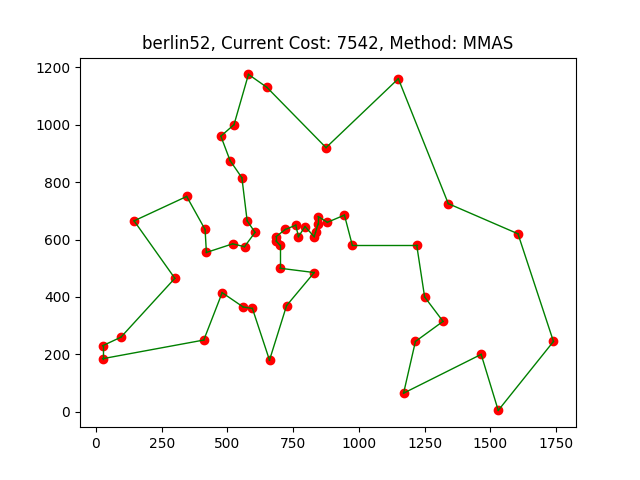
\includegraphics[width=0.95\linewidth]{figure/mmas_berlin52}
	\caption{The optimal solution of berlin52 given by MMAS}
	\label{fig:mmasberlin52}
\end{figure}

\begin{figure}[H]
	\centering
	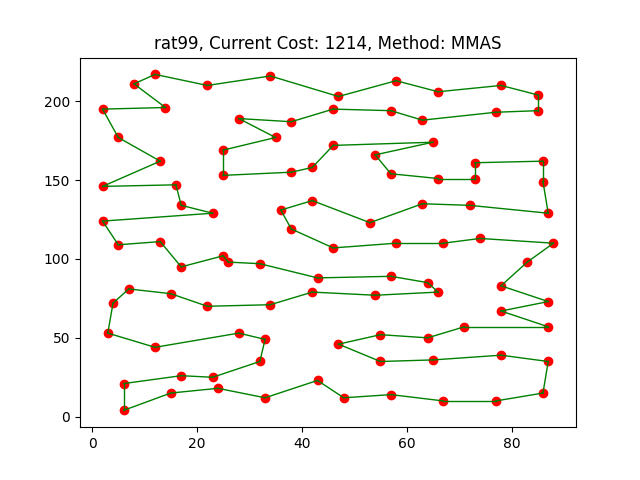
\includegraphics[width=0.95\linewidth]{figure/mass_rat99}
	\caption{The optimal solution of rat99 given by MMAS}
	\label{fig:massrat99}
\end{figure}

\begin{figure}[H]
	\centering
	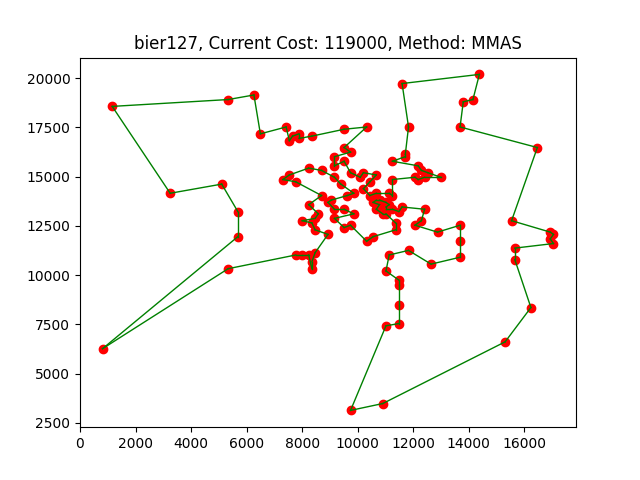
\includegraphics[width=0.95\linewidth]{figure/mmas_bier127}
	\caption{The optimal solution of bier127 given by MMAS}
	\label{fig:mmasbier127}
\end{figure}

\begin{figure}[H]
	\centering
	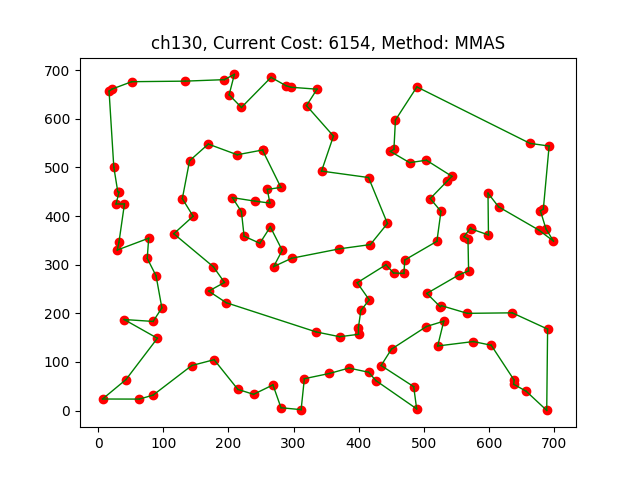
\includegraphics[width=0.95\linewidth]{figure/mmas_ch130}
	\caption{The optimal solution of ch130 given by MMAS}
	\label{fig:mmasch130}
\end{figure}

\begin{figure}[H]
	\centering
	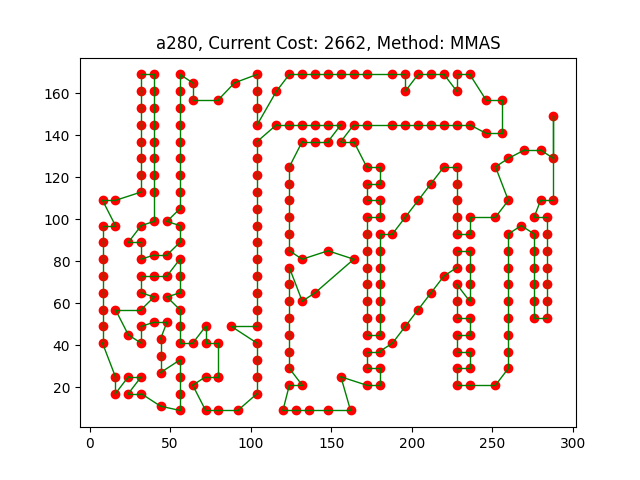
\includegraphics[width=0.95\linewidth]{figure/mmas_a280}
	\caption{The optimal solution of a280 given by MMAS}
	\label{fig:mmasa280}
\end{figure}




\subsubsection{Solutions of firefly}

\begin{figure}[H]
	\centering
	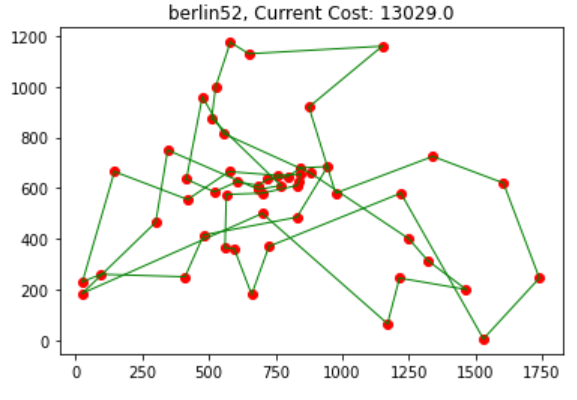
\includegraphics[width=0.95\linewidth]{figure/fire_berlin52}
	\caption{The optimal solution of berlin52 given by firefly algorithms}
	\label{fig:fireberlin52}
\end{figure}

\begin{figure}[H]
	\centering
	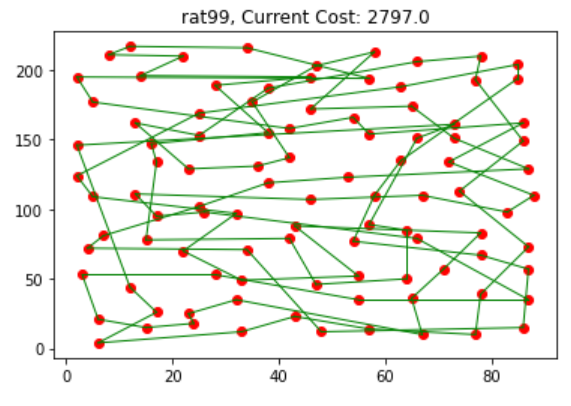
\includegraphics[width=0.95\linewidth]{figure/fire_rat99}
	\caption{The optimal solution of rat99 given by firefly algorithms}
	\label{fig:firerat99}
\end{figure}

\begin{figure}[H]
	\centering
	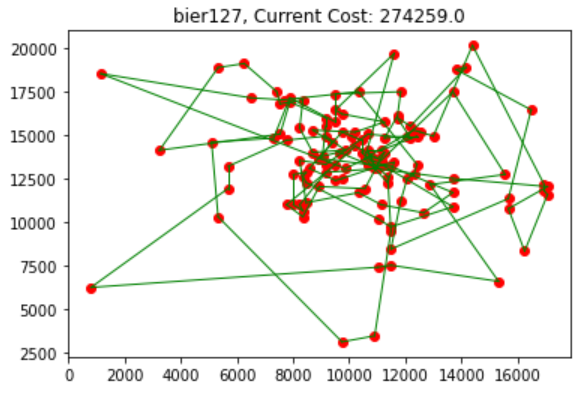
\includegraphics[width=0.95\linewidth]{figure/fire_bier127}
	\caption{The optimal solution of bier127 given by firefly algorithms}
	\label{fig:firebier127}
\end{figure}

\begin{figure}[H]
	\centering
	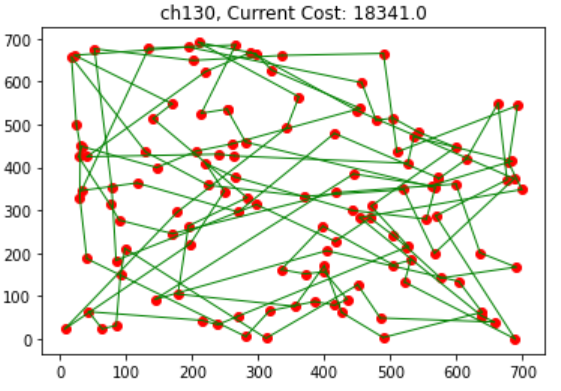
\includegraphics[width=0.95\linewidth]{figure/fire_ch130}
	\caption{The optimal solution of ch130 given by firefly algorithms}
	\label{fig:firech130}
\end{figure}

\begin{figure}[H]
	\centering
	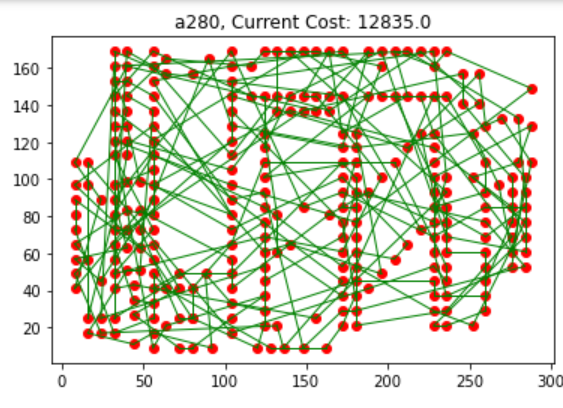
\includegraphics[width=0.95\linewidth]{figure/fire_a280}
	\caption{The optimal solution of a280 given by firefly algorithms}
	\label{fig:firea280}
\end{figure}


\begin{table*}[b]
	\caption{The solutions of five TSP instances given by MMAS, RL and Firefly.}
	\label{tab: results}
	\resizebox{\textwidth}{!}{%
		\begin{tabular}{@{}ccccccccc@{}}
			\toprule
			\textbf{Problem} &
			\textbf{Method} &
			\textbf{Avg. Distance} &
			\textbf{Std. Distance} &
			\textbf{Avg. Time (sec.)} &
			\textbf{Best Distance} &
			\textbf{Worst Distance} &
			\textbf{Relative Diff. (\%)} &
			\textbf{Optimal Distance} \\ \midrule
			\multirow{3}{*}{berlin52} & RL      & 9841.4            & 212.3       & 0.34     & 9075   & 10074  & 30.49          & \multirow{3}{*}{7542}   \\
			& MMAS    & \textbf{7542}     & 0           & 6.90 & 7542   & 7542   & \textbf{0}           &                         \\
			& Firefly & 11541.2           & 1046.2      & 33.01       & 9520   & 12321  & 53.03         &                         \\
			\multirow{3}{*}{rat99}    & RL      & 1578.6            & 70.34       & 0.16        & 1465   & 1697   & 30.36        & \multirow{3}{*}{1211}   \\
			& MMAS    & \textbf{1226.2}   & 7.43 & 428.65  & 1214   & 1234   & \textbf{1.26} &                         \\
			& Firefly & 2915.6            & 278.44    & 59.72       & 2604   & 3440   & 140.76          &                         \\
			\multirow{3}{*}{bier127}  & RL      & 221276.6          & 3125.08     & 0.2096      & 216331 & 224186 & 87.08         & \multirow{3}{*}{118282} \\
			& MMAS    & \textbf{119981.8} & 277.35  & 632.72 & 119700 & 120365 & \textbf{1.44} &                         \\
			& Firefly & 272727.6          & 8591.6      & 85.98       & 261526 & 286210 & 130.57        &                         \\
			\multirow{3}{*}{ch130}    & RL      & 7989.6            & 385.75      & 0.214       & 7330   & 8529   & 30.76          & \multirow{3}{*}{6110}   \\
			& MMAS    & \textbf{6211}     & 34.34 & 657.71 & 6154   & 6240   & \textbf{1.65} &                         \\
			& Firefly & 18001.8           & 847.49      & 68.81      & 16940  & 19055  & 194.63          &                         \\
			\multirow{3}{*}{a280}     & RL      & 12828.2           & 181.05     & 0.8         & 12459  & 13049  & 397.41          & \multirow{3}{*}{2579}   \\
			& MMAS    & \textbf{2685.6}   & 20.26 & 2553.39 & 2662   & 2718   & \textbf{4.13} &                         \\
			& Firefly & 12791.4           & 366.47      & 134.7       & 12189  & 12189  & 395.98          &                         \\ \bottomrule
		\end{tabular}%
	}
\end{table*}


\section{Discussion}

\section{Conclusion}



\printbibliography


\end{document}